\documentclass{article}
\usepackage[utf8]{inputenc}

% Page setup
\usepackage[a4paper,landscape,margin=2cm]{geometry}
\usepackage{amsmath}

% Typography
\usepackage[scaled]{helvet}
\let\familydefault\sfdefault

\usepackage[usenames,svgnames]{xcolor}
\usepackage{tikz,pgfplots}
\usetikzlibrary{positioning,arrows,intersections,calc}

\definecolor{coloractor}    {RGB}{199,212,104}
\definecolor{colormediator} {RGB}{ 79,142,209}
\definecolor{colorbus}      {RGB}{143,232,186}
\definecolor{colortext}     {RGB}{ 29, 29, 27}
\definecolor{coloraction}   {RGB}{129, 29, 27}
\definecolor{colortest}     {RGB}{129,129,227}

\begin{document}
\pagestyle{empty}
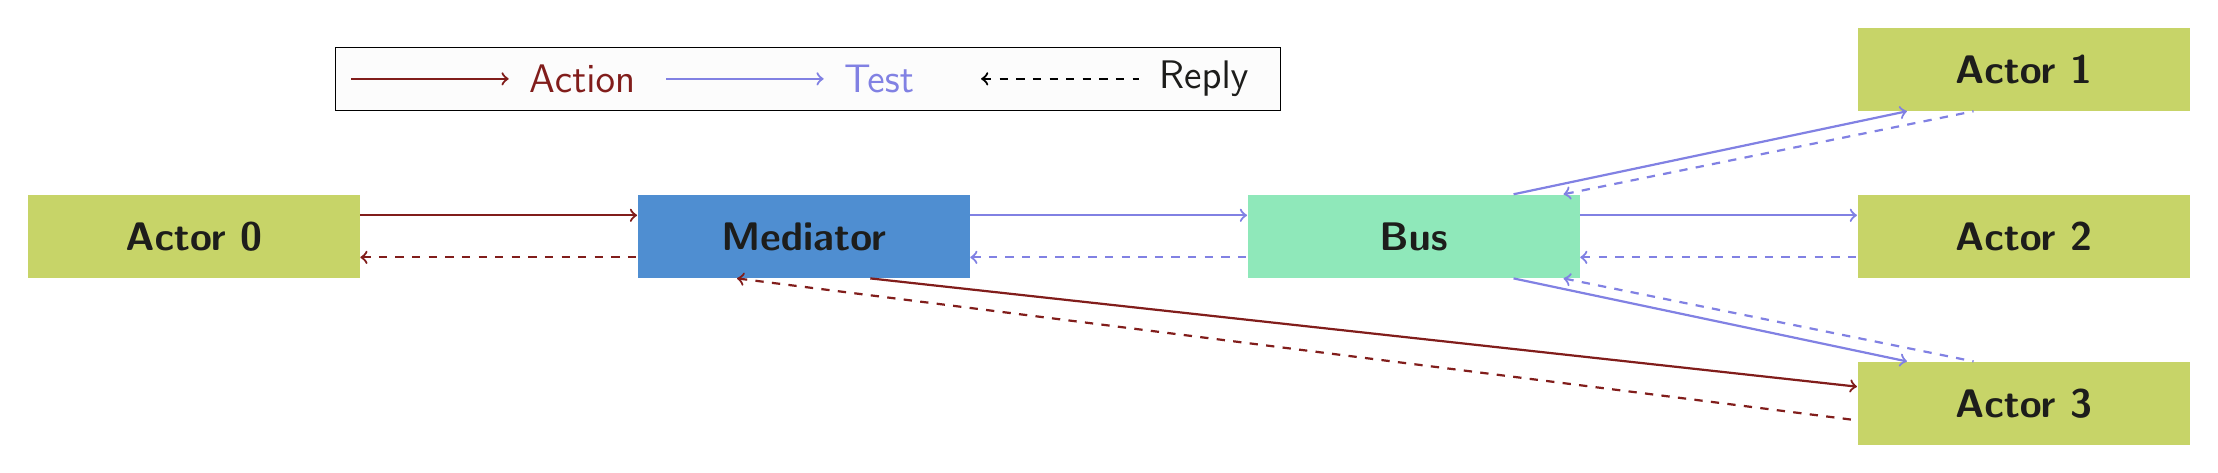
\begin{tikzpicture}[
    node distance = 10em, auto,
    font={\Large\itshape},
    base/.style={text=colortext,font={\Large\bfseries},inner sep=10pt,align=center,rectangle},
    txt/.style={text=colortext,font={},inner sep=7pt,align=center},
    action/.style={txt,color=coloraction},
    test/.style={txt,color=colortest},
    treenode/.style={base,thick,draw=colortext,text width=2em},
    relation/.style={text width=13em},
]

    \node[base,fill=coloractor,text width=10em]                    (actor0)   {Actor 0};
    
    \node[base,fill=colormediator,text width=10em,right=of actor0] (mediator) {Mediator};
    
    \node[base,fill=colorbus,text width=10em,right=of mediator]   (bus)       {Bus};
    
    \node[base,fill=coloractor,text width=10em,right=of bus]      (actor1)    {Actor 2};
    \node[base,fill=coloractor,text width=10em,above=3em of actor1]   (actor2)    {Actor 1};
    \node[base,fill=coloractor,text width=10em,below=3em of actor1]   (actor3)    {Actor 3};
    
    \draw[action,->,thick]($(actor0.north east)!0.5!(actor0.east)$) -- ($(mediator.north west)!0.5!(mediator.west)$);
    \draw[action,<-,thick,dashed]($(actor0.south east)!0.5!(actor0.east)$) -- ($(mediator.south west)!0.5!(mediator.west)$);
    
    \draw[test,->,thick]($(mediator.north east)!0.5!(mediator.east)$) -- ($(bus.north west)!0.5!(bus.west)$);
    \draw[test,<-,thick,dashed]($(mediator.south east)!0.5!(mediator.east)$) -- ($(bus.south west)!0.5!(bus.west)$);
    
    \draw[test,->,thick]($(bus.north east)!0.5!(bus.east)$) -- ($(actor1.north west)!0.5!(actor1.west)$);
    \draw[test,<-,thick,dashed]($(bus.south east)!0.5!(bus.east)$) -- ($(actor1.south west)!0.5!(actor1.west)$);
    \draw[test,->,thick]($(bus.north east)!0.4!(bus.north)$) -- ($(actor2.south)!0.7!(actor2.south west)$);
    \draw[test,<-,thick,dashed]($(bus.north east)!0.1!(bus.north)$) -- ($(actor2.south)!0.3!(actor2.south west)$);
    \draw[test,->,thick]($(bus.south east)!0.4!(bus.south)$) -- ($(actor3.north)!0.7!(actor3.north west)$);
    \draw[test,<-,thick,dashed]($(bus.south east)!0.1!(bus.south)$) -- ($(actor3.north)!0.3!(actor3.north west)$);
    
    \draw[action,->,thick]($(mediator.south east)!0.3!(mediator.south west)$) -- ($(actor3.north west)!0.6!(actor3.west)$);
    \draw[action,<-,thick,dashed]($(mediator.south east)!0.7!(mediator.south west)$) -- ($(actor3.south west)!0.6!(actor3.west)$);
    
    % Legend
    %\draw [fill=black!1!white] (1.8,4.3) rectangle (5.4,1.7);
    %\draw[action,->,thick]     (2,4) -- (4,4) node[right] {Action};
    %\draw[test,->,thick]       (2,3) -- (4,3) node[right] {Test};
    %\draw[txt,<-,thick,dashed] (2,2) -- (4,2) node[right] {Reply};
    
    \draw [fill=black!1!white] (1.8,1.6) rectangle (13.8,2.4);
    \draw[action,->,thick,font={\Large}]     (2,2) -- (4,2) node[right] {Action};
    \draw[test,->,thick,font={\Large}]       (6,2) -- (8,2) node[right] {Test};
    \draw[txt,<-,thick,dashed,font={\Large}] (10,2) -- (12,2) node[right] {Reply};

\end{tikzpicture}
\end{document}
